\bgroup
\begin{frame}{DQN in Atari}
\begin{itemize}
\item End-to-end learning of values $Q(s, a)$ from pixels $s$
\item Input state $s$ is stack of raw pixels from last 4 frames
\item Output is $Q(s, a)$ for 18 joystick/button positions
\item Reward is change in score for that step
\end{itemize}
\begin{figure}
\centering
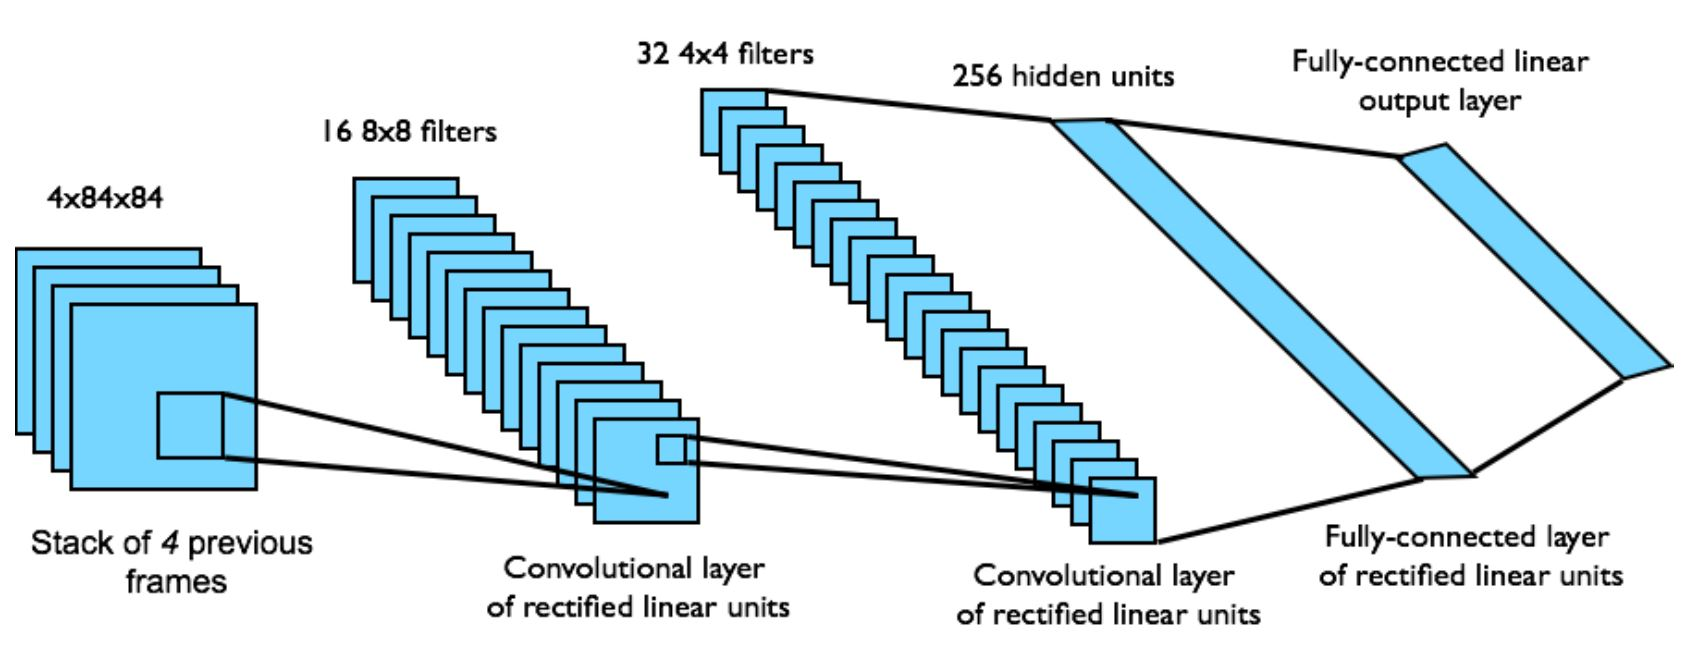
\includegraphics[width=0.8\textwidth]{img/dqn.JPG}
\end{figure}
\end{frame}
\egroup